% =============================================================================
% REPORT SECTIONS v3 (Methodology -> Discussion). Paste in place of the old ones.
% Preamble needs: booktabs, longtable, float, array, amsmath, graphicx, xcolor,
%                 url, tikz (positioning, arrows.meta), pgfplots (compat=1.17)
% All numbers come from thesis_dbp/reports/ (P2 session E, X1, X2, X3a-c, DIV2K).
% =============================================================================

% =============================================================================
\section{Proposed Methodology}
\label{sec:method}
% =============================================================================

The detector combines three evidence modules that look at an image in different ways (Figure~\ref{fig:pipeline}). All three use the same DINOv3 ViT-B/16 backbone and native-resolution crops (no resizing), so that differences between them come from the \textit{evidence}, not from model size.

\begin{figure}[H]
\centering
\noindent\resizebox{\linewidth}{!}{%
\begin{tikzpicture}[
    font=\small,
    box/.style={draw, rounded corners=2pt, align=center, minimum height=12mm, text width=3.6cm, fill=#1},
    box/.default=white,
    arr/.style={-{Stealth[length=2mm]}, thick}
]
\node[box=gray!12, text width=2.4cm] (in) {\textbf{Input image}\\native resolution,\\no resizing};
\node[box=blue!8, right=14mm of in] (s2) {\textbf{S2: Learned artifact}\\DINOv3-B + LoRA\\trained on aligned\\real/reconstruction pairs};
\node[box=blue!8, above=5mm of s2] (s1) {\textbf{S1: Semantic}\\frozen DINOv3-B\\+ linear probe};
\node[box=blue!8, below=5mm of s2] (s3) {\textbf{S3: Decoder-bank probe}\\12 decoders, 8 lineages\\20 features per decoder\\+ trained head};
\node[box=orange!15, right=14mm of s2] (fu) {\textbf{Fusion}\\fixed-weight,\\real-normalised mean};
\node[box=green!12, right=12mm of fu, text width=2.6cm] (out) {\textbf{Score}\\real / AI-generated};
\draw[arr] (in.east) -- (s1.west);
\draw[arr] (in.east) -- (s2.west);
\draw[arr] (in.east) -- (s3.west);
\draw[arr] (s1.east) -- (fu.west);
\draw[arr] (s2.east) -- (fu.west);
\draw[arr] (s3.east) -- (fu.west);
\draw[arr] (fu.east) -- (out.west);
\end{tikzpicture}%
}%
\caption{Overview of the detector: three evidence modules and their fusion.}
\label{fig:pipeline}
\end{figure}

\begin{itemize}
    \item \textbf{S1 -- Semantic module.} A frozen DINOv3-B encoder gives a 1,536-dimensional embedding; a logistic-regression probe classifies it. S1 looks at \textit{what} the image shows and how natural it looks.
    \item \textbf{S2 -- Learned artifact module.} The same backbone is adapted with LoRA (rank 8, 589,824 trainable parameters) on \textit{aligned} pairs: a real photograph and the same photograph passed through a decoder. Because the content is identical, the only learnable difference is the decoder trace.
    \item \textbf{S3 -- Decoder-bank probe.} At test time, the image is encoded and decoded by every decoder in the bank (Table~\ref{tab:bank}). The change $x - D_k(E_k(x))$ is summarised by 20 features per decoder (PSNR, mean residual, LPIPS, a 16-bin residual spectrum, high-frequency ratio). A trained head (S3-Set: shared per-decoder network with attention pooling; S3-LR: logistic regression) turns the 12 responses into one score.
    \item \textbf{Fusion.} Each module's score is normalised against real validation images only, $z_k = \operatorname{clip}\big((s_k - \operatorname{med}_k^{\mathrm{real}})/(1.4826\,\operatorname{MAD}_k^{\mathrm{real}}), -5, 5\big)$, and the fused score is the mean $F = \frac{1}{3}(z_{\mathrm{S1}} + z_{\mathrm{S2}} + z_{\mathrm{S3}})$.
\end{itemize}

\begin{table}[H]
\centering
\footnotesize
\caption{The decoder bank used by S2 (training) and S3 (test-time probe): 12 distinct decoders from 8 lineages.}
\label{tab:bank}
\begin{tabular}{>{\raggedright\arraybackslash}p{3.0cm} >{\raggedright\arraybackslash}p{4.6cm} c >{\raggedright\arraybackslash}p{4.4cm}}
\toprule
\textbf{Lineage} & \textbf{Decoders} & \textbf{Latent ch.} & \textbf{Generators that use it} \\
\midrule
KL 4-ch (SD1) & sd15, sd21, sd\_ft\_ema & 4 & SD1.x, SD2.x, PixArt-$\alpha$ \\
KL 4-ch (SDXL) & sdxl, sdxl\_fp16fix & 4 & SDXL, Playground v2.5, HunyuanDiT \\
KL 16-ch & sd35, flux & 16 & SD3/3.5, FLUX.1 \\
KL 16-ch (Qwen) & qwen & 16 & Qwen-Image \\
KL 32-ch (FLUX.2) & flux2\_klein & 32 & FLUX.2 \\
Deep compression & dcae & 32 & SANA \\
VQ tokenizer & movq & 4 & Kandinsky / token-based models \\
GAN super-resolution & realesrgan\_x4 & -- & GAN upscalers \\
\bottomrule
\end{tabular}
\end{table}

\noindent\textbf{Two training settings are compared throughout.} The \textit{prior approach} trains only with the SD1 decoder family, as in published aligned-training detectors (Aligned Datasets, ICLR 2025; DDA, NeurIPS 2025; SEF, 2026). \textit{Our approach} trains with all 12 decoders of the bank. Everything else (backbone, LoRA, data, augmentation, crops) is identical.

\newpage
% =============================================================================
\section{Preliminary Experiments and Failure Analysis}
% =============================================================================

Before DBP, three approaches were implemented and evaluated. Each failed for a reason that could be measured, and each failure directly shaped the proposed design. Their pipelines are summarised in Figure~\ref{fig:prior}.

\begin{figure}[H]
\centering
\includegraphics[width=0.95\linewidth]{images/Prior_Approaches.png}
\caption{Pipelines of the approaches tried or compared against, and the point at which each one breaks.}
\label{fig:prior}
\end{figure}

\subsection{Frequency-Domain Ensemble (FFT, DCT and Related Transforms)}

\subsubsection{Setup}

The first approach extracted 25 spectral features per image. These included radial FFT power, a high-frequency energy ratio, spectral slope, and $8\times8$ block-DCT band energies. The features were classified in two ways. The first was a training-free mathematical classifier with a per-feature Youden-$J$ threshold. The second was a small MLP that learns which frequency evidence to trust, so that the model effectively selects the most discriminative frequency band. The classifiers were evaluated on a balanced set of 1{,}000 images (Stable Diffusion faces vs.\ FFHQ real faces) in a Kaggle notebook. An earlier local run used a mixed set covering approximately 12 generators.

\subsubsection{Why the Frequency Ensemble Fails}

The MLP outperformed the mathematical classifier in-domain. However, there is no stable frequency signature for the model to select, for four measured reasons.

\begin{enumerate}
    \item \textbf{The sign of the gap depends on content.} Two real photographs were passed through the same SD-1.5 VAE. For one, the reconstruction has \textit{less} high-frequency power than the real image; for the other it has \textit{more} (Figure~\ref{fig:spectral}, left). A threshold or learned band weight that is correct for one image is wrong for the other.
    \item \textbf{Ordinary processing erases the gap.} After JPEG ($q=75$), the high-frequency FFT gap keeps only 7\% of its magnitude and the DCT high-band gap reverses sign. A $0.5\times$ resize removes 98\% of the spectral-slope gap (Figures~\ref{fig:spectral} and~\ref{fig:gap}).
    \item \textbf{On benchmarks, the spectral signal is largely compression history.} In the MLLM benchmark (E3), reals are JPEG while 93.7\% of fakes are never-compressed PNG. A one-line rule on JPEG quality scores 96.4\% against a 66.7\% baseline (Section~\ref{sec:shortcuts}). DCT and FFT features observe exactly this $8\times8$ block structure.
    \item \textbf{Modern decoders leave weaker traces.} The 16-channel VAEs of SD3.5 and FLUX reconstruct far more faithfully (LPIPS 0.029--0.039) than 4-channel SD-family VAEs (0.075--0.090). The artefact therefore shrinks exactly on the generators that most need to be detected.
\end{enumerate}

\begin{figure}[H]
\centering
\includegraphics[width=0.95\linewidth]{images/Spectral_Gap.png}
\caption{Fake-minus-real radial FFT power for SD-1.5 VAE reconstructions. Left: the sign of the high-frequency gap flips between two photographs. Right: JPEG $q{=}75$ and $0.5\times$ resize collapse the gap. Computed from the P0 smoke-test images ($n=2$ photographs); the figure illustrates the mechanism and is not a statistical result.}
\label{fig:spectral}
\end{figure}

\begin{figure}[H]
\centering
\includegraphics[width=0.85\linewidth]{images/Gap_Retention.png}
\caption{Share of the clean real-vs-fake feature gap that survives degradation. Negative values mean the sign flipped, so a learned rule would vote the wrong way.}
\label{fig:gap}
\end{figure}

\subsection{FIRE Baseline Reproduction}
\label{sec:fire_repro}

FIRE (CVPR 2025) was reproduced on Kaggle from the official checkpoints. It achieved $\sim$100\% in-domain, which confirms that the pipeline is correct. Zero-shot on modern generators, it collapsed (Table~\ref{tab:fire}, Figure~\ref{fig:fire}). At threshold 0.5, accuracy equals $n_{\text{fake}}/(n_{\text{fake}}+389)$ on every generator, meaning that all 389 real images are labelled fake. On SD v1.4, AUC was 40.0\% (95\% CI 34.9--45.2), which is an inverted ranking.

\begin{table}[H]
\centering
\caption{FIRE zero-shot results at threshold 0.5.}
\label{tab:fire}
\begin{tabular}{l c c c}
\toprule
\textbf{Generator} & \textbf{Fakes / Reals} & \textbf{Accuracy (\%)} & \textbf{Observation} \\
\midrule
FLUX & 392 / 389 & 50.19 & all reals called fake \\
SDXL & 300 / 389 & 43.54 & all reals called fake \\
Lumina & 300 / 389 & 43.54 & all reals called fake \\
SD3.5 & 300 / 389 & 43.54 & all reals called fake \\
SD v1.4 & 161 / 389 & 29.27 & AUC 40.0 [34.9, 45.2] \\
\bottomrule
\end{tabular}
\end{table}

\begin{figure}[H]
\centering
\includegraphics[width=0.75\linewidth]{images/FIRE_ZeroShot.png}
\caption{FIRE zero-shot accuracy equals the share of fakes, i.e.\ every real image is called fake.}
\label{fig:fire}
\end{figure}

The cause is the training signal. FIRE reconstructs with the SD-1.5 VAE, but its ResNet-50 head was trained on ADM fakes. ADM is a pixel-space model with no VAE, so the head never learned a decoder fingerprint; it learned LSUN-vs-ADM cues instead. FIRE also resizes the short side to 256~px, which discards most decoder evidence in 1024~px images. DBP therefore trains on fakes that pass through real decoders, aligned with their real counterparts, at native resolution.

\subsection{Hidden Shortcuts in Public Benchmarks}
\label{sec:shortcuts}

Each evaluation set was audited by measuring the accuracy of the best rule that looks only at a single JPEG parameter. Three of the five labelled sets carry such a shortcut. Two of these were invisible to a simple ``is it compressed?'' check (Figure~\ref{fig:shortcut}, Table~\ref{tab:shortcut}). All results in this report use the matched views built to remove these shortcuts.

\begin{figure}[H]
\centering
\includegraphics[width=0.9\linewidth]{images/Benchmark_Shortcuts.png}
\caption{Accuracy of a one-line compression rule before and after the matched views built in this work. The E7 FLUX.1 subset cannot be corrected, because chroma subsampling is destructive, so it is reported only in its luma-only form.}
\label{fig:shortcut}
\end{figure}

\begin{table}[H]
\centering
\footnotesize
\caption{Accuracy of the best single encoding-parameter rule (\%), before and after matching. A lift above 5 points is a shortcut.}
\label{tab:shortcut}
\begin{tabular}{>{\raggedright\arraybackslash}p{3.8cm} c c c c >{\raggedright\arraybackslash}p{3.0cm}}
\toprule
\textbf{Set} & \textbf{Rows} & \textbf{Baseline} & \textbf{Raw rule} & \textbf{After match} & \textbf{Reporting rule} \\
\midrule
E3 MLLM (GPT-Image-2, Nano-Banana-2) & 2{,}178 & 66.67 & 96.42 & 66.90 & matched view \\
E4 WildRF (social media) & 2{,}503 & 50.02 & 75.43 & 61.41 & upper bound only \\
E5 Chameleon & 26{,}033 & 57.09 & 60.22 & 57.32 & pipeline-matched view \\
E7 DDA-COCO, FLUX.1 subset & 9{,}971 & 50.15 & 100.00 & 100.00 & luma-only view \\
\bottomrule
\end{tabular}
\end{table}

\newpage
% =============================================================================
\section{Experimental Setup}
\label{sec:setup}
% =============================================================================

\textbf{Training data.} 2,417 real MS-COCO \texttt{train2017} images, their reconstructions by the bank decoders (48,132 aligned pairs), and 2,488 SD1.5 generations (format-matched). Dataset details and licences are given in Section~\ref{sec:datasets}.

\textbf{Test sets} (never used for training; 11,775-image test panel, plus validation images):
\begin{itemize}
    \item \textbf{Validation reconstructions:} 491 held-out real COCO images vs.\ their reconstructions by each of the 12 decoders.
    \item \textbf{E3:} GPT-Image-2 and Nano-Banana-2 (newest closed generators), also split by content: texture, structure (text, documents, user interfaces) and hybrid.
    \item \textbf{E4 WildRF} (social-media images) and \textbf{E5 Chameleon} (hard, human-indistinguishable AI images).
    \item \textbf{E7 DDA-COCO:} real photographs that only passed through a generator's VAE (SDXL, SD3.5, FLUX.1 luma-only).
    \item \textbf{DIV2K:} lossless real photographs, used to measure false alarms.
\end{itemize}

\textbf{Metrics.}
\begin{itemize}
    \item \textbf{AUC:} how well a module ranks fakes above reals (0.5 = chance, 1.0 = perfect).
    \item \textbf{Detected at 5\% FPR:} the share of fakes caught when only 5\% of that test set's real images are wrongly flagged.
    \item \textbf{False alarms:} the share of \textit{real} images flagged as fake at the threshold fixed on validation (COCO) images.
\end{itemize}
95\% bootstrap confidence intervals (1,000 resamples) are given in brackets. ``Unseen'' means the generator or decoder was not used in training.


\newpage
% =============================================================================
\section{Results}
\label{sec:results}
% =============================================================================

This section reports the experimental results of the three modules, first one at a time and then combined. For each module we first show how it performs on its own, then where it fails, and, where we changed the method, how the change improves it. The section ends with the fusion of the three modules and a short summary of the findings.

All modules are evaluated on exactly the same images. Two kinds of test data are used (Section~\ref{sec:setup}). The \textit{validation reconstructions} are real COCO photographs and the same photographs after passing through each of the 12 decoders; they show whether a module recognises the trace of each decoder. The \textit{test panel} contains images from generators that were never used in training: the newest closed generators GPT-Image-2 and Nano-Banana-2 (E3), social-media images (E4 WildRF), hard human-curated images (E5 Chameleon) and VAE-only reconstructions (E7 DDA-COCO). Three numbers are reported. The \textbf{AUC} measures how well a module ranks fake images above real ones (0.5 means guessing, 1.0 means perfect). \textbf{Detected at 5\% FPR} is the share of fakes caught when only 5\% of the real images of that test set may be wrongly flagged. \textbf{False alarms} is the share of real images flagged as fake at the threshold fixed on COCO validation images.

% -----------------------------------------------------------------------------
\subsection{Module S1: Frozen DINOv3 with a Linear Probe}
\label{sec:res_s1}
% -----------------------------------------------------------------------------

S1 is the simplest module. The image is passed through the frozen DINOv3-B encoder, and a linear classifier decides from the resulting embedding whether the image is real or fake. Because the encoder is frozen, S1 can only use what a general-purpose vision model already sees: the content, structure and overall appearance of the image. This subsection first reports how S1 performs on its own (Table~\ref{tab:s1}) and then examines where and why it fails (Table~\ref{tab:s1fail}).

\subsubsection{S1 Results}

Table~\ref{tab:s1} lists S1's performance on every test set. The first four rows are generators that S1 never saw in training: the two closed generators of E3, the social-media images of E4 and the Chameleon set (E5). The next three rows are DDA-COCO images, i.e.\ real COCO photographs that were only passed through the VAE of SDXL, SD3.5 or FLUX.1. The DIV2K row contains only real, lossless photographs, so only the false-alarm rate can be measured on it. The last row is the average over the seven unseen test sets.

\begin{table}[H]
\centering
\small
\caption{S1 alone on the test sets (trained on SD1-family data).}
\label{tab:s1}
\begin{tabular}{>{\raggedright\arraybackslash}p{4.3cm} >{\centering\arraybackslash}p{3.4cm} >{\centering\arraybackslash}p{2.6cm} >{\centering\arraybackslash}p{2.6cm}}
\toprule
\textbf{Test set} & \textbf{AUC [95\% CI]} & \textbf{Detected at 5\% FPR} & \textbf{False alarms on reals} \\
\midrule
E3 GPT-Image-2 & 0.435 [0.399, 0.474] & 3.6\% & 60.2\% \\
E3 Nano-Banana-2 & 0.512 [0.477, 0.551] & 7.2\% & 60.2\% \\
E4 WildRF & 0.784 [0.761, 0.805] & 29.9\% & 65.1\% \\
E5 Chameleon & 0.561 [0.542, 0.580] & 9.1\% & 67.4\% \\
E7 SDXL VAE (VAE-only) & 0.878 [0.857, 0.899] & 47.3\% & 6.2\% \\
E7 SD3.5 VAE (VAE-only) & 0.822 [0.794, 0.847] & 34.7\% & 6.2\% \\
E7 FLUX.1 VAE (VAE-only, luma) & 0.657 [0.624, 0.692] & 11.4\% & 21.0\% \\
DIV2K lossless real photos & -- & -- & 53.5\% \\
\midrule
\textbf{Average (7 unseen sets)} & \textbf{0.664 [0.650, 0.678]} & \textbf{20.4\%} & -- \\
\bottomrule
\end{tabular}
\end{table}

S1 performs reasonably only where fake images differ visibly from real ones. It reaches an AUC of 0.784 on WildRF and 0.82--0.88 on the SDXL and SD3.5 reconstructions. On the newest closed generators, however, it is no better than guessing: 0.435 on GPT-Image-2, which is below chance, and 0.512 on Nano-Banana-2. At a 5\% false-positive rate it catches only 3.6\% and 7.2\% of these images, and 20.4\% of all unseen fakes on average.

The last column reveals a second problem. The decision threshold was fixed on COCO validation images, where it wrongly flags 5\% of real images (6.2\% on the COCO reals of E7). On real images from other sources, the same threshold flags 60--67\% of internet photographs and 53.5\% of lossless DIV2K photographs as fake. S1 has therefore learned what COCO photographs look like rather than what makes an image real, so its scores do not transfer to new sources of real images.

\subsubsection{Where S1 Fails}

Table~\ref{tab:s1} already shows two failures: the closed generators and the false alarms on real images from other sources. A third failure needs its own experiment. A latent-diffusion image carries two kinds of traces: \textit{generation} traces, left by the diffusion model that invents the content, and \textit{decoder} traces, left by the VAE decoder that turns the latent code into pixels. To find out which of the two S1 relies on, a frozen DINOv3-B probe was trained only on real COCO images against \textit{fully generated} SD1.5 images, with no reconstructions in training. It was then tested on real photographs that had only been passed through one decoder. These images carry decoder traces but no generation traces, because their content is real. Table~\ref{tab:s1fail} reports the result for every decoder in the bank.

\begin{table}[H]
\centering
\small
\caption{S1 failure on decoder-only images: a frozen DINOv3-B probe trained on full generations only, tested on held-out images (491 reals).}
\label{tab:s1fail}
\begin{tabular}{>{\raggedright\arraybackslash}p{6.2cm} c c}
\toprule
\textbf{Fake images} & \textbf{AUC} & \textbf{Detected at 5\% FPR} \\
\midrule
SD1.5 full generations (same kind as training) & 0.999 & 99.8\% \\
\midrule
\multicolumn{3}{l}{\textit{Real photographs reconstructed by one decoder (VAE-only)}} \\
sd15 & 0.893 & 45.8\% \\
movq & 0.887 & 42.2\% \\
qwen & 0.854 & 32.2\% \\
sd\_ft\_ema & 0.819 & 36.9\% \\
sd21 & 0.813 & 33.6\% \\
sdxl & 0.796 & 26.3\% \\
dcae & 0.783 & 23.6\% \\
sd35 & 0.721 & 16.5\% \\
flux & 0.708 & 15.7\% \\
\textbf{flux2\_klein (FLUX.2)} & \textbf{0.546} & \textbf{5.9\%} \\
\midrule
realesrgan\_x4 (GAN upscaler, not a VAE) & 0.996 & 97.4\% \\
\bottomrule
\end{tabular}
\end{table}

On fully generated images, which carry both kinds of traces, the probe is almost perfect (AUC 0.999, 99.8\% detected). On real photographs that only passed through a decoder, it drops sharply: it catches only 16--46\% of them at a 5\% false-positive rate, and only 5.9\% for FLUX.2, the most faithful decoder in the bank, where its AUC of 0.546 is close to guessing. The only exception is Real-ESRGAN (97.4\%), a GAN upscaler that visibly changes textures rather than leaving a fine decoder trace.

This shows that S1 recognises generated images through their \textit{generation} traces, not through the \textit{decoder} traces. Images that were edited or re-rendered through a latent-diffusion decoder, and fakes whose content looks natural, therefore escape S1. This gap is the reason for the two decoder-based modules, S2 and S3.

% -----------------------------------------------------------------------------
\subsection{Module S2: Learned Decoder Artifacts}
\label{sec:res_s2}
% -----------------------------------------------------------------------------

S2 uses the same DINOv3-B backbone as S1, but adapts it with LoRA so that it can learn the fine traces that decoders leave in the pixels. It is trained on aligned pairs: a real photograph and the same photograph after passing through a decoder. Because both images show exactly the same content, the only difference the model can learn is the decoder trace. This subsection first reproduces the training used in published aligned-training detectors and shows where it fails (Table~\ref{tab:s2prior}). It then reports the effect of our change, training with the 12-decoder bank (Table~\ref{tab:s2ours}, Figure~\ref{fig:s2}).

\subsubsection{Prior Approach: Training with One Decoder Family}

Aligned Datasets (ICLR 2025), DDA (NeurIPS 2025) and SEF (2026) all build their training reconstructions with one Stable Diffusion VAE family. To measure the limits of this design under identical conditions, S2 was first trained in the same way, using only the SD1 decoder family. Table~\ref{tab:s2prior} reports the result in two parts. The upper part uses the validation reconstructions, which show how far the learned decoder trace carries over to the other decoders of the bank. The lower part uses the unseen test sets, including the E3 images split by content type: texture (natural scenes), structure (text, documents and user interfaces) and hybrid images.

\begin{table}[H]
\centering
\small
\caption{S2 trained with one decoder family (prior approach).}
\label{tab:s2prior}
\begin{tabular}{>{\raggedright\arraybackslash}p{5.0cm} c c c}
\toprule
\textbf{Test} & \textbf{AUC} & \textbf{Detected at 5\% FPR} & \textbf{False alarms on reals} \\
\midrule
\multicolumn{4}{l}{\textit{Validation: real vs.\ reconstructions by each decoder}} \\
SD1 family (seen in training) & 1.000 & 100\% & -- \\
SDXL, DC-AE, MoVQ, Real-ESRGAN & 0.997--1.000 & 99.0--100\% & -- \\
SD3.5 & 0.974 & 81.3\% & -- \\
FLUX.1 & 0.929 & 56.6\% & -- \\
Qwen-Image & 0.855 & 27.1\% & -- \\
\textbf{FLUX.2} & \textbf{0.598} & \textbf{7.1\%} & -- \\
\midrule
\multicolumn{4}{l}{\textit{Test sets (unseen generators)}} \\
E3 GPT-Image-2 & 0.492 & 2.8\% & 68.8\% \\
E3 Nano-Banana-2 & 0.723 & 21.2\% & 68.8\% \\
E3 texture images & 0.840 & 40.3\% & 38.9\% \\
E3 structure images & 0.476 & 2.8\% & 82.7\% \\
E3 hybrid images & 0.479 & 4.8\% & 80.1\% \\
E4 WildRF & 0.955 & 82.9\% & 83.0\% \\
E5 Chameleon & 0.685 & 21.1\% & 83.9\% \\
\bottomrule
\end{tabular}
\end{table}

The upper part of Table~\ref{tab:s2prior} shows a clear pattern. Decoders of the training family, and older or lower-fidelity decoders (SDXL, DC-AE, MoVQ, Real-ESRGAN), are detected almost perfectly (AUC 0.997--1.000). As decoders become more faithful, detection falls steadily: SD3.5 0.974, FLUX.1 0.929, Qwen-Image 0.855, and FLUX.2 0.598, where only 7.1\% of the reconstructions are caught. A detector trained on one decoder family therefore cannot be trusted on the newest decoders, which are exactly the ones used by current generators.

The lower part shows the same weakness on real generators. S2 is strong on WildRF (0.955) and on texture images (0.840), but it is below chance on GPT-Image-2 (0.492) and at chance on structure and hybrid images (0.476 and 0.479). In addition, 69--84\% of the real images of E3, E4 and E5 are flagged as fake at the validation threshold.

\subsubsection{What We Add: Training with the 12-Decoder Bank}

Our change is the set of training decoders. Instead of one SD family, S2 is trained on reconstructions by \textbf{all 12 decoders from 8 lineages} (Table~\ref{tab:bank}), including the 16-channel (SD3.5, FLUX.1, Qwen-Image), 32-channel (FLUX.2), deep-compression (DC-AE), VQ and GAN decoders that the prior approach never sees. Backbone, LoRA, data, augmentation and crops are unchanged, so every difference between the two versions is caused by the decoder bank.

Table~\ref{tab:s2ours} puts the two versions side by side on the same images. The first block repeats the four modern decoders on which the prior approach failed. The second block lists the unseen test sets, followed by their average. The last row gives the false-alarm rates on the real images of E3, E4 and E5. Each cell gives the AUC and, in brackets, the share of fakes detected at a 5\% false-positive rate.

\begin{table}[H]
\centering
\small
\caption{Updated S2 (12-decoder bank) vs.\ the prior approach. AUC, with detection at 5\% FPR in brackets.}
\label{tab:s2ours}
\begin{tabular}{>{\raggedright\arraybackslash}p{4.2cm} c c c}
\toprule
\textbf{Test} & \textbf{Prior (1 family)} & \textbf{Ours (12 decoders)} & \textbf{Change (AUC)} \\
\midrule
\multicolumn{4}{l}{\textit{Validation: real vs.\ reconstructions}} \\
FLUX.2 & 0.598 (7.1\%) & \textbf{0.982 (90.2\%)} & $+0.384$ \\
Qwen-Image & 0.855 (27.1\%) & \textbf{0.999 (99.4\%)} & $+0.144$ \\
FLUX.1 & 0.929 (56.6\%) & \textbf{0.995 (97.8\%)} & $+0.066$ \\
SD3.5 & 0.974 (81.3\%) & \textbf{0.999 (99.8\%)} & $+0.025$ \\
\midrule
\multicolumn{4}{l}{\textit{Test sets (unseen by both)}} \\
E3 GPT-Image-2 & 0.492 (2.8\%) & \textbf{0.663 (17.6\%)} & $+0.171$ \\
E3 Nano-Banana-2 & 0.723 (21.2\%) & \textbf{0.825 (42.6\%)} & $+0.102$ \\
E3 texture images & 0.840 (40.3\%) & \textbf{0.928 (63.1\%)} & $+0.088$ \\
E3 structure images & 0.476 (2.8\%) & \textbf{0.608 (12.6\%)} & $+0.132$ \\
E3 hybrid images & 0.479 (4.8\%) & \textbf{0.667 (11.8\%)} & $+0.188$ \\
E4 WildRF & \textbf{0.955 (82.9\%)} & 0.927 (68.9\%) & $-0.028$ \\
E5 Chameleon & 0.685 (21.1\%) & 0.681 (15.1\%) & $-0.004$ \\
\midrule
\textbf{Average of E3--E5 (4 sets)} & 0.714 & \textbf{0.774} & $\mathbf{+0.060}$ \\
\midrule
\multicolumn{4}{l}{\textit{False alarms on real images}} \\
E3 / E4 / E5 reals & 68.8 / 83.0 / 83.9\% & \textbf{33.3 / 61.2 / 48.9\%} & lower \\
\bottomrule
\end{tabular}
\end{table}

Figure~\ref{fig:s2} shows the main rows of Table~\ref{tab:s2ours} as a chart. Grey bars are the prior approach and blue bars are S2 trained on the 12-decoder bank. The four groups on the left are modern decoders (validation), the four on the right are unseen test sets, and the dashed line marks chance (AUC 0.5).

\begin{figure}[H]
\centering
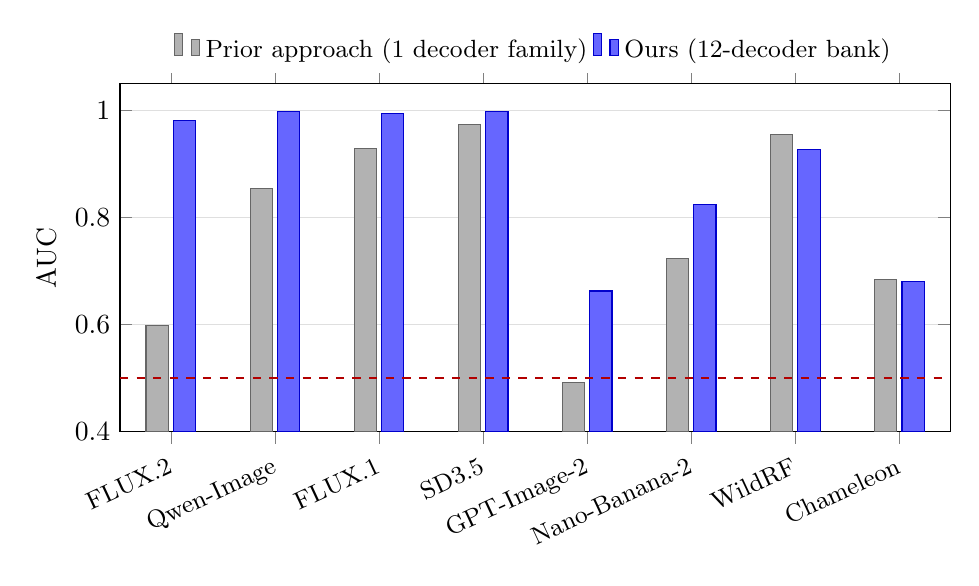
\begin{tikzpicture}
\begin{axis}[
    ybar, bar width=8pt, width=\linewidth, height=6cm,
    ymin=0.4, ymax=1.05, ylabel={AUC},
    symbolic x coords={FLUX.2,Qwen-Image,FLUX.1,SD3.5,GPT-Image-2,Nano-Banana-2,WildRF,Chameleon},
    xtick=data, x tick label style={font=\small, rotate=25, anchor=north east},
    enlarge x limits=0.07, ymajorgrids, grid style={gray!25},
    legend style={at={(0.5,1.03)}, anchor=south, legend columns=2, draw=none, font=\small},
]
\addplot[fill=gray!60, draw=gray!80!black] coordinates {(FLUX.2,0.598) (Qwen-Image,0.855) (FLUX.1,0.929) (SD3.5,0.974) (GPT-Image-2,0.492) (Nano-Banana-2,0.723) (WildRF,0.955) (Chameleon,0.685)};
\addplot[fill=blue!60, draw=blue!80!black] coordinates {(FLUX.2,0.982) (Qwen-Image,0.999) (FLUX.1,0.995) (SD3.5,0.999) (GPT-Image-2,0.663) (Nano-Banana-2,0.825) (WildRF,0.927) (Chameleon,0.681)};
\draw[dashed, red!70!black, thick] ({rel axis cs:0,0}|-{axis cs:FLUX.2,0.5}) -- ({rel axis cs:1,0}|-{axis cs:FLUX.2,0.5});
\legend{Prior approach (1 decoder family), Ours (12-decoder bank)}
\end{axis}
\end{tikzpicture}
\caption{S2: prior approach vs.\ our 12-decoder training. Left four: validation reconstructions; right four: unseen test sets. Dashed line: chance.}
\label{fig:s2}
\end{figure}

Training on the 12-decoder bank removes the failure on modern decoders. FLUX.2 rises from 0.598 to 0.982, and its detection rate from 7.1\% to 90.2\%; Qwen-Image, FLUX.1 and SD3.5 all reach 0.995--0.999. These decoders are part of the bank, so this block shows that S2 can learn all decoder families at once without losing the old ones; a leave-one-lineage-out study will test decoders that are completely unseen.

The test sets were not seen by either version, so they measure real generalisation. The two newest closed generators improve clearly (GPT-Image-2 $+0.171$, Nano-Banana-2 $+0.102$), as do all three E3 content types ($+0.088$ to $+0.188$). The average over the four unseen test sets rises from 0.714 to 0.774. False alarms on real images also fall substantially, from 68.8/83.0/83.9\% to 33.3/61.2/48.9\% on E3/E4/E5.

The change does not solve everything. WildRF drops slightly (0.955 to 0.927) and Chameleon does not improve (0.681). At a 5\% false-positive rate only 15--69\% of the unseen fakes are caught, and false alarms remain high (33--61\% on internet reals and 53.5\% on DIV2K). These remaining failures are the target of the next phase.

% -----------------------------------------------------------------------------
\subsection{Module S3: Decoder-Bank Probe}
\label{sec:res_s3}
% -----------------------------------------------------------------------------

S3 uses the decoders themselves as forensic probes at test time. Each test image is encoded and decoded by every decoder of the bank, and the change between the input and the output is described by 20 features per decoder. An image that was produced through a decoder of a given family changes little when it passes through that family again, whereas a natural photograph changes more. This subsection answers two questions: is one decoder enough, and if not, how should the responses of many decoders be combined?

Figure~\ref{fig:residuals} shows what S3 measures. Each panel is the difference between a real photograph and its reconstruction by one decoder, amplified ten times. The residual energy concentrates on fine detail such as hair, fabric and edges, and its pattern differs between decoder families: the VAE residuals resemble each other, whereas the GAN upscaler leaves a clearly different pattern. These differences are what S3's features capture.

\begin{figure}[H]
\centering
\includegraphics[width=0.85\linewidth]{images/Residual_Maps.png}
\caption{Residual maps ($\times10$) of a real photograph after passing through bank decoders. The VAE and GAN residuals are visibly different families.}
\label{fig:residuals}
\end{figure}

\subsubsection{One Decoder, and More Decoders Without Training}

The simplest form of S3 uses a single decoder and needs no training: an image is scored by how little it changes under reconstruction, measured with the LPIPS distance (as in AEROBLADE, CVPR 2024). Table~\ref{tab:s3naive} compares two versions of this score. The first column uses one decoder, sd15. The second column uses all 11 VAE decoders and keeps the smallest distance over the bank, which is the natural way to extend the score to many decoders without training. The upper block tests reconstructions by each decoder; an asterisk marks the cases in which the decoder that made the fake is part of the score. The lower block reports the test sets.

\begin{table}[H]
\centering
\small
\caption{S3 with a single decoder pass vs.\ eleven decoder passes combined without training (AUC). $^{*}$ = the decoder that made the fake is used by the score.}
\label{tab:s3naive}
\begin{tabular}{>{\raggedright\arraybackslash}p{5.2cm} c c}
\toprule
\textbf{Fake images} & \textbf{1 decoder (sd15)} & \textbf{11 decoders, no training} \\
\midrule
\multicolumn{3}{l}{\textit{Validation: reconstructions by each decoder}} \\
sd15 & \textbf{0.993}$^{*}$ & 0.588$^{*}$ \\
sd21 & 0.871 & 0.594$^{*}$ \\
sd\_ft\_ema & 0.834 & 0.534$^{*}$ \\
sdxl & 0.758 & 0.661$^{*}$ \\
sdxl\_fp16fix & 0.762 & 0.682$^{*}$ \\
dcae & 0.686 & 0.503$^{*}$ \\
movq & 0.693 & 0.601$^{*}$ \\
sd35 & 0.588 & 0.717$^{*}$ \\
qwen & 0.615 & 0.839$^{*}$ \\
flux & 0.576 & \textbf{0.955}$^{*}$ \\
flux2\_klein & 0.594 & \textbf{0.979}$^{*}$ \\
realesrgan\_x4 & 0.887 & 0.933 \\
\midrule
\multicolumn{3}{l}{\textit{Test sets}} \\
E3 GPT-Image-2 & 0.562 & 0.623 \\
E3 Nano-Banana-2 & 0.596 & 0.599 \\
E4 WildRF & 0.675 & 0.473 \\
E5 Chameleon & 0.664 & 0.685 \\
E7 SDXL VAE & 0.696 & 0.560 \\
E7 SD3.5 VAE & 0.563 & 0.598 \\
E7 FLUX.1 VAE (luma) & 0.516 & 0.635 \\
\bottomrule
\end{tabular}
\end{table}

With one decoder, the score works only for that decoder's own reconstructions (AUC 0.993 for sd15) and for its close relatives (sd21 0.871, sd\_ft\_ema 0.834). On the 16- and 32-channel decoders (SD3.5, FLUX, Qwen-Image, FLUX.2) it is close to guessing (0.576--0.615), and on the test sets it stays between 0.52 and 0.70. One decoder therefore covers one family only.

Adding the other decoders without training does not fix this. Taking the smallest distance over all 11 VAEs makes the high-fidelity decoders detectable (FLUX 0.955, FLUX.2 0.979, Qwen-Image 0.839), but it destroys the score for every other decoder: sd15 falls from 0.993 to 0.588, DC-AE to 0.503, and WildRF to 0.473. The reason is that the high-fidelity decoders also reconstruct \textit{real} photographs almost perfectly. When the smallest distance is taken, real images receive the same low distance as fakes, and the signal of the matching decoder is lost. Simply passing images through more decoders is therefore not enough; their responses must be combined by a trained head.

\subsubsection{Our Approach: Twelve Decoders with a Trained Head}

To measure how a trained head uses additional decoders, S3's two heads (S3-LR and S3-Set) were retrained with the responses of $k$ decoders, from $k=1$ (sd15 only) to $k=12$ (the whole bank), while the training images were kept fixed. Decoders were added one lineage at a time in a fixed order (second column of Table~\ref{tab:s3k}). For each head, the table reports three AUCs: on the validation reconstructions of all 12 decoders; on reconstructions by decoders whose responses the head does not yet use (``unseen-feature decoders'', which exist only for $k<12$); and on the unseen generators of E3--E5.

\begin{table}[H]
\centering
\footnotesize
\caption{S3 with a trained head as the number of decoders grows (AUC). Validation: reals vs.\ reconstructions by all 12 decoders. Unseen-feature decoders: decoders whose responses the head does not use. Unseen generators: E3 (GPT-Image-2, Nano-Banana-2), E4 WildRF and E5 Chameleon.}
\label{tab:s3k}
\setlength{\tabcolsep}{4pt}
\begin{tabular}{c >{\raggedright\arraybackslash}p{3.4cm} cc cc cc}
\toprule
& & \multicolumn{2}{c}{\textbf{Validation}} & \multicolumn{2}{c}{\textbf{Unseen-feature dec.}} & \multicolumn{2}{c}{\textbf{Unseen gen.\ (E3--E5)}} \\
\cmidrule(lr){3-4}\cmidrule(lr){5-6}\cmidrule(lr){7-8}
$k$ & \textbf{Decoders added} & S3-LR & S3-Set & S3-LR & S3-Set & S3-LR & S3-Set \\
\midrule
1 & sd15 & 0.810 & 0.831 & 0.775 & 0.799 & 0.648 & 0.650 \\
2 & + sdxl & 0.851 & 0.852 & 0.815 & 0.805 & 0.675 & 0.643 \\
4 & + movq, sd35 & 0.900 & 0.907 & 0.858 & 0.851 & 0.654 & 0.631 \\
6 & + qwen, flux2\_klein & 0.941 & 0.943 & 0.924 & 0.897 & 0.626 & 0.626 \\
8 & + dcae, realesrgan\_x4 & 0.950 & 0.936 & 0.934 & 0.828 & 0.628 & 0.625 \\
\textbf{12} & + sd21, sd\_ft\_ema, sdxl\_fp16fix, flux & \textbf{0.973} & \textbf{0.984} & -- & -- & 0.638 & 0.604 \\
\bottomrule
\end{tabular}
\end{table}

Figure~\ref{fig:s3k} plots the same numbers against the number of decoders. Solid lines show the validation AUC on decoder reconstructions; dashed lines show the unseen generators of E3--E5.

\begin{figure}[H]
\centering
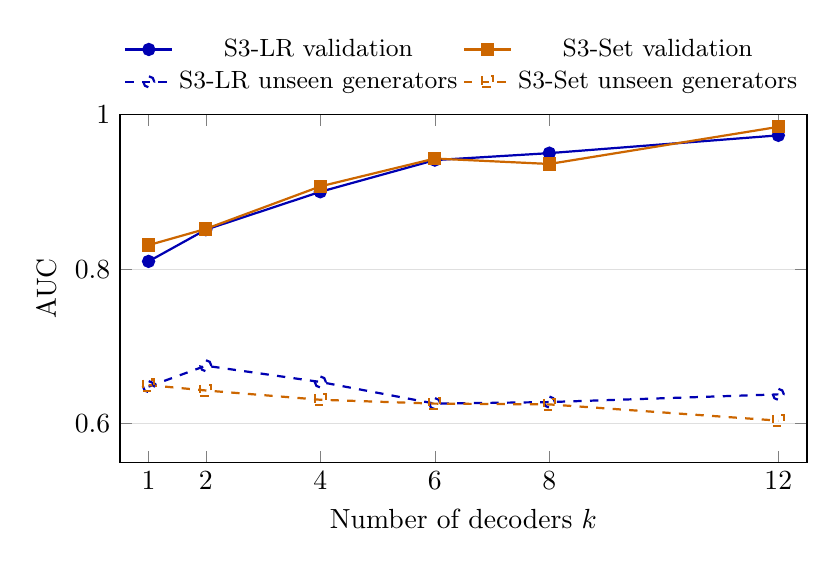
\begin{tikzpicture}
\begin{axis}[
    width=0.85\linewidth, height=6cm,
    xmin=0.5, xmax=12.5, ymin=0.55, ymax=1.0,
    xtick={1,2,4,6,8,12}, xlabel={Number of decoders $k$}, ylabel={AUC},
    ymajorgrids, grid style={gray!25},
    legend style={at={(0.5,1.03)}, anchor=south, legend columns=2, draw=none, font=\small},
]
\addplot[thick, blue!70!black, mark=*] coordinates {(1,0.810) (2,0.851) (4,0.900) (6,0.941) (8,0.950) (12,0.973)};
\addplot[thick, orange!80!black, mark=square*] coordinates {(1,0.831) (2,0.852) (4,0.907) (6,0.943) (8,0.936) (12,0.984)};
\addplot[thick, dashed, blue!70!black, mark=o] coordinates {(1,0.648) (2,0.675) (4,0.654) (6,0.626) (8,0.628) (12,0.638)};
\addplot[thick, dashed, orange!80!black, mark=square] coordinates {(1,0.650) (2,0.643) (4,0.631) (6,0.626) (8,0.625) (12,0.604)};
\legend{S3-LR validation, S3-Set validation, S3-LR unseen generators, S3-Set unseen generators}
\end{axis}
\end{tikzpicture}
\caption{S3 with a trained head: AUC as decoders are added. Solid: validation reconstructions; dashed: unseen generators (E3--E5).}
\label{fig:s3k}
\end{figure}

With a trained head, every additional decoder helps on decoder reconstructions, which is the opposite of the untrained minimum in Table~\ref{tab:s3naive}. Validation AUC rises steadily from 0.810 (S3-LR) and 0.831 (S3-Set) with one decoder to \textbf{0.973 and 0.984 with all twelve}. The head also becomes better at recognising reconstructions from decoders whose responses it does not use (S3-LR: 0.775 with one decoder to 0.934 with eight). This shows that the responses of different decoders carry shared information about decoder traces in general, which a trained head can exploit but a simple minimum cannot.

The dashed lines show the limit of this module. On the unseen generators of E3--E5, adding decoders does not help: S3-LR stays between 0.626 and 0.675, and S3-Set falls slightly from 0.650 to 0.604. The bank recognises decoder traces, but the closed generators in these sets use decoders that are not in the bank, and the matched views of these sets are JPEG-compressed, which likely weakens the fine residual traces that S3 measures.

% -----------------------------------------------------------------------------
\subsection{Fusion of S1, S2 and S3}
\label{sec:res_fusion}
% -----------------------------------------------------------------------------

The previous subsections show that the three modules look at different evidence: S1 at generation traces, S2 at learned decoder traces, and S3 at the responses of the decoder bank. This subsection tests whether combining them gives a better detector than the best module alone. Each module's score is first normalised against real validation images, and the normalised scores are then averaged with equal weights (Section~\ref{sec:method}). The same procedure is applied to every pair of modules. A version with weights learned on validation data is also reported.

Table~\ref{tab:fusion_sets} shows, for each unseen test set, the AUC of each module alone and of the three modules fused, using the final modules trained with the 12-decoder bank. The last column names the best of the four.

\begin{table}[H]
\centering
\small
\caption{Each module alone and the three fused, per unseen test set (AUC; 12-decoder training).}
\label{tab:fusion_sets}
\begin{tabular}{>{\raggedright\arraybackslash}p{3.6cm} cccc l}
\toprule
\textbf{Test set} & \textbf{S1} & \textbf{S2} & \textbf{S3} & \textbf{S1+S2+S3} & \textbf{Best} \\
\midrule
E3 GPT-Image-2 & 0.467 & \textbf{0.663} & 0.623 & 0.623 & S2 \\
E3 Nano-Banana-2 & 0.563 & \textbf{0.825} & 0.557 & 0.708 & S2 \\
E3 texture images & 0.624 & \textbf{0.928} & 0.691 & 0.874 & S2 \\
E3 structure images & 0.525 & 0.608 & 0.626 & \textbf{0.653} & fusion \\
E3 hybrid images & 0.422 & \textbf{0.667} & 0.423 & 0.503 & S2 \\
E4 WildRF & 0.794 & \textbf{0.927} & 0.554 & 0.856 & S2 \\
E5 Chameleon & 0.635 & 0.681 & 0.684 & \textbf{0.738} & fusion \\
\midrule
\textbf{Average (E3--E5, 4 sets)} & 0.615 & \textbf{0.774} & 0.604 & 0.731 & S2 \\
\bottomrule
\end{tabular}
\end{table}

S2 is the best module on five of the seven test sets, often by a wide margin (Nano-Banana-2 0.825, texture images 0.928, WildRF 0.927). S1 and S3 are much weaker on these sets, and when their scores are averaged with S2 they pull the fused score down: on Nano-Banana-2 from 0.825 to 0.708, and on WildRF from 0.927 to 0.856.

Fusion wins only on the two sets where S2 is weakest. On structure images (text, documents, interfaces) the fused score reaches 0.653 against 0.626 for the best single module, and on Chameleon it reaches 0.738 against 0.684, a gain of 5.4 points. On these sets the modules make different mistakes, so combining them helps. Averaged over the four sets, however, the fused score (0.731) remains below S2 alone (0.774).

Table~\ref{tab:fusion} extends this comparison to every combination of modules and to both training settings, averaged over the unseen test sets. The first setting, with one decoder family, is the pre-registered test of the fusion hypothesis: fusion had to beat the best single module by at least 2 points, with a 95\% confidence interval excluding zero. For each combination, the table gives the average AUC, its difference from S2 in AUC points (with a 95\% bootstrap confidence interval for the combinations), and the average share of fakes detected at a 5\% false-positive rate.

\begin{table}[H]
\centering
\footnotesize
\caption{All combinations averaged over the unseen test sets (7 sets for one-family training, 4 for the 12-decoder bank). AUC, change vs.\ S2 in points [95\% CI], and detection at 5\% FPR.}
\label{tab:fusion}
\setlength{\tabcolsep}{3.5pt}
\begin{tabular}{>{\raggedright\arraybackslash}p{2.6cm} ccc ccc}
\toprule
& \multicolumn{3}{c}{\textbf{Training: 1 decoder family (pre-registered)}} & \multicolumn{3}{c}{\textbf{Training: 12-decoder bank}} \\
\cmidrule(lr){2-4}\cmidrule(lr){5-7}
\textbf{Module(s)} & \textbf{AUC} & \textbf{vs S2 [95\% CI]} & \textbf{Det.} & \textbf{AUC} & \textbf{vs S2 [95\% CI]} & \textbf{Det.} \\
\midrule
S1 & 0.664 & $-14.0$ & 20.4\% & 0.615 & $-15.9$ & 12.7\% \\
\textbf{S2} & \textbf{0.804} & -- & \textbf{47.6\%} & \textbf{0.774} & -- & \textbf{36.1\%} \\
S3 & 0.682 & $-12.2$ & 18.1\% & 0.604 & $-17.0$ & 3.2\% \\
\midrule
S1 + S2 & 0.725 & $-7.9$ [$-8.9$, $-6.8$] & 26.9\% & 0.725 & $-4.9$ [$-6.1$, $-3.6$] & 28.9\% \\
S1 + S3 & 0.716 & $-8.8$ [$-10.1$, $-7.6$] & 26.2\% & 0.652 & $-12.2$ [$-14.2$, $-10.0$] & 8.9\% \\
S2 + S3 & 0.735 & $-6.9$ [$-8.0$, $-5.8$] & 29.9\% & 0.738 & $-3.6$ [$-5.2$, $-2.1$] & 15.6\% \\
\textbf{S1 + S2 + S3} & 0.745 & $\mathbf{-5.9}$ [$-6.9$, $-4.9$] & 34.1\% & 0.731 & $\mathbf{-4.3}$ [$-5.9$, $-2.7$] & 20.8\% \\
S1 + S2 + S3, learned weights & 0.557 & $-24.7$ [$-26.2$, $-23.0$] & 10.3\% & 0.745 & $-2.9$ [$-4.5$, $-1.2$] & 19.8\% \\
\bottomrule
\end{tabular}
\end{table}

The answer is the same in both settings: no combination beats S2 alone. Fusing all three modules costs 5.9 AUC points with one-family training and 4.3 points with the 12-decoder bank, and every confidence interval lies entirely below zero. Pairs behave the same way; the best pair, S2+S3, is still 3.6--6.9 points below S2. Learned weights do not help either. With one-family training they collapse to 0.557, because on the easy validation images one weak head received almost all of the weight; with the 12-decoder bank they remain 2.9 points below S2. The pre-registered decision is therefore \textbf{NO-GO}, and the result was the same for both training seeds ($-5.89$ and $-5.03$ points).

Figure~\ref{fig:fusion} summarises the same averages. Grey bars are one-family training and blue bars are the 12-decoder bank. In both settings the S2 bar is the highest, and every bar that combines S1 or S3 with S2 is lower than S2 alone.

\begin{figure}[H]
\centering
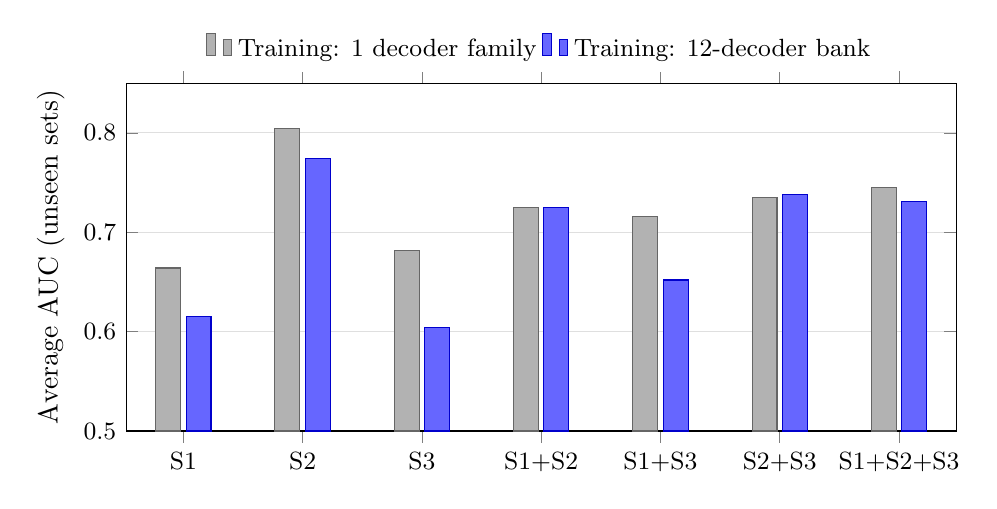
\begin{tikzpicture}
\begin{axis}[
    ybar, bar width=9pt, width=\linewidth, height=6cm,
    ymin=0.5, ymax=0.85, ylabel={Average AUC (unseen sets)},
    symbolic x coords={S1,S2,S3,S1+S2,S1+S3,S2+S3,S1+S2+S3},
    xtick=data, tick label style={font=\small},
    enlarge x limits=0.08, ymajorgrids, grid style={gray!25},
    legend style={at={(0.5,1.03)}, anchor=south, legend columns=2, draw=none, font=\small},
]
\addplot[fill=gray!60, draw=gray!80!black] coordinates {(S1,0.664) (S2,0.804) (S3,0.682) (S1+S2,0.725) (S1+S3,0.716) (S2+S3,0.735) (S1+S2+S3,0.745)};
\addplot[fill=blue!60, draw=blue!80!black] coordinates {(S1,0.615) (S2,0.774) (S3,0.604) (S1+S2,0.725) (S1+S3,0.652) (S2+S3,0.738) (S1+S2+S3,0.731)};
\legend{Training: 1 decoder family, Training: 12-decoder bank}
\end{axis}
\end{tikzpicture}
\caption{Average AUC of each module and each combination. S2 alone is the highest in both training settings.}
\label{fig:fusion}
\end{figure}

Two reasons explain why fusion does not help on average. First, S1 and S3 are much weaker than S2 on most unseen sets (12--17 AUC points lower on average), so giving them equal weight dilutes S2's stronger evidence. Second, the modules often miss the same images: the overlap between the sets of images missed by two modules is 54--70\% (Jaccard index), so even a perfect per-image choice of module would add only 4--7 points. The useful complementarity is local, on Chameleon and on structure images, and a fixed average cannot exploit it. S2 trained on the 12-decoder bank is therefore the main detector, while S1 and S3 remain useful evidence for these specific cases.

% -----------------------------------------------------------------------------
\subsection{Summary}
% -----------------------------------------------------------------------------

The main results of this section are:

\begin{enumerate}
    \item \textbf{S1} detects fully generated images (99.8\%) but misses images that only passed through a decoder (6--46\%), and it fails on the closed generators.
    \item \textbf{S2, prior approach} (one decoder family) fails on modern decoders (FLUX.2: 0.598) and on GPT-Image-2 (0.492). \textbf{Our 12-decoder training} fixes the modern decoders (FLUX.2: 0.982), improves GPT-Image-2 ($+0.171$) and Nano-Banana-2 ($+0.102$), and lowers false alarms.
    \item \textbf{S3:} one decoder recognises only its own reconstructions; adding decoders without training makes things worse; \textbf{twelve decoders with a trained head} recognise all decoder families (0.97--0.98). It does not yet help on unseen closed generators.
    \item \textbf{Fusion:} the three modules fused do \textit{not} beat S2 on average (NO-GO), but fusion helps on Chameleon and structure images. S2 trained on the 12-decoder bank is therefore the main detector.
    \item \textbf{Main open problem:} false alarms on real internet photographs (33--61\% for updated S2). Fixing this calibration is the next phase.
\end{enumerate}

\newpage
% =============================================================================
\section{Datasets}
\label{sec:datasets}
% =============================================================================

The corpus is split strictly by role. Training data consists only of real images and their decoder reconstructions or generations. Evaluation sets are never used for training, and every one is audited for compression shortcuts and checked for leakage against the training manifests. Licence terms are recorded because the detector has a deployment goal.

\subsection{Training and Control Data}

\begin{longtable}{p{2.9cm} p{2.3cm} p{2.4cm} p{6.6cm}}
\toprule
\textbf{Dataset} & \textbf{Type} & \textbf{Size used} & \textbf{Description / Role} \\
\midrule
\endhead
MS-COCO 2017 (\texttt{train2017}) & Real images & 2{,}417 & Real class for training (T-real). Deliberately restricted to \texttt{train2017}, because the DDA-COCO evaluation reals are COCO \texttt{val2017}. JPEG, estimated quality 90--96. \\
\midrule
DIV2K (train HR) & Real images, lossless & 1{,}594 crops (800 photos) & Control set (T-ctrl): lossless PNG reals that show whether a model relies on JPEG structure. Diagnostic only; academic-use licence. \\
\midrule
DBP reconstruction pairs & Aligned fakes & 48{,}132 & Each real reconstructed by the 12 distinct bank decoders at native crop 384. Built in this work. \\
\midrule
SD-1.5 generations & Generated images & 2{,}488 (+ matched) & Text-to-image generations from COCO captions, each with a JPEG-matched variant. Built in this work. \\
\bottomrule
\end{longtable}

\subsection{Evaluation Benchmarks}

\begin{longtable}{p{2.9cm} p{2.3cm} p{2.4cm} p{6.6cm}}
\toprule
\textbf{Dataset} & \textbf{Type} & \textbf{Size used} & \textbf{Description / Role} \\
\midrule
\endhead
E7 DDA-COCO & Image, VAE reconstructions & 34{,}969 (5{,}000 real) & \textbf{Primary head-to-head set.} COCO \texttt{val2017} reconstructed by six VAEs (SD2.1, SD ft-EMA, SD ft-MSE, SDXL, SD3.5, FLUX.1). Directly comparable with SEF and DDA. Apache-2.0. \\
\midrule
E8 EvalGEN & Image, generated & 5{,}000 (fakes only) & Five 2024--2025 generators, three of them not diffusion models; 1{,}000 per generator by seeded stratified sampling. Reported as a detection rate at FPR-calibrated thresholds. Apache-2.0. \\
\midrule
E3 MLLM set & Image, commercial & 2{,}178 (726 real) & GPT-Image-2 and Nano-Banana-2 against real images, split into texture, structure (text, documents, UI) and hybrid content. Reported in Raw, JPEG-matched (primary) and Preprocessing views. Apache-2.0. \\
\midrule
E4 WildRF (test) & Image, social media & 2{,}503 & Reddit, Twitter and Facebook images; in-the-wild compression. Research-only licence; results are upper bounds because a quality shortcut remains. \\
\midrule
E5 Chameleon & Image, hard fakes & 26{,}033 (14{,}863 real) & Human-hard AI images from the AIDE work. Evaluated at a 320~px crop through a pipeline-matched view. Academic use only. \\
\midrule
E6 MNW (Microsoft) & Evaluation-only benchmark & pending & Microsoft--Northwestern--WITNESS benchmark with periodically added new generators. Access granted; download route pending. Evaluation-only, no training. \\
\bottomrule
\end{longtable}

\subsection{Dataset Sources}

\begin{itemize}
    \item \textbf{MS-COCO 2017} \\ \url{https://cocodataset.org}
    \item \textbf{DIV2K} \\ \url{https://data.vision.ee.ethz.ch/cvl/DIV2K/}
    \item \textbf{DDA-COCO (E7)} \\ \url{https://huggingface.co/datasets/Junwei-Xi/DDA-COCO}
    \item \textbf{EvalGEN (E8)} \\ \url{https://huggingface.co/datasets/Junwei-Xi/EvalGEN}
    \item \textbf{WildRF (E4)} \\ \url{https://github.com/barcavia/RealTime-DeepfakeDetection-in-the-RealWorld}
    \item \textbf{Chameleon (E5)} \\ \url{https://github.com/shilinyan99/AIDE}
    \item \textbf{MLLM set (E3)} \\ \url{https://huggingface.co/datasets/zr-zhang/} \\ \url{MLLM-Generated-Image-Detection-Dataset}
    \item \textbf{MNW (E6)} \\ \url{https://github.com/microsoft/MNW}
\end{itemize}

% =============================================================================
\section{Limitations and Next Steps}
\label{sec:limitations}
% =============================================================================

\begin{itemize}
    \item \textbf{Seen decoders.} The 12-decoder S2 has seen every bank decoder in training; a leave-one-lineage-out study will test truly unseen decoders.
    \item \textbf{False alarms.} Thresholds set on COCO reals do not transfer to internet photographs. More diverse real training images and calibration on a few target-platform reals are the next step.
    \item \textbf{Analyses after the decision.} Only the fusion test with one-family training was pre-registered; the other comparisons were computed afterwards on the same test panel and explain, but do not change, that decision.
    \item \textbf{Backbone and data size.} ViT-B/16 and 2,417 real training images were used because of the T4 compute budget; a ViT-L check is planned.
\end{itemize}
